Langkah-langkah untuk instalasi XAMPP adalah sebagai berikut :

\begin{enumerate}

	\item Tentunya mengunduh \textit{installer} aplikasi ini dari alamat \url{https://www.apachefriends.org}, pilihlah yang model \textit{installer} agar lebih mudah proses instalasinya.
	
	\item Awal proses instalasi, kita akan bertemu dengan tampilan seperti pada gambar \ref{fig:01-03-01-001} berikut ini :
	
	\begin{figure}[H]
		\centering
		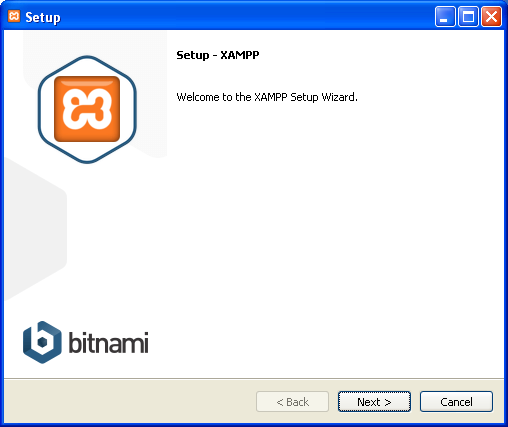
\includegraphics[width=1\textwidth]{01-03-01-001-start-install-xampp}
		\caption{Awal Instalasi XAMPP}
		\label{fig:01-03-01-001}
	\end{figure}
	
	\item Setelah itu kita diminta untuk memilih komponen yang akan ikut di\textit{install} / dipasangkan seperti pada gambar \ref{fig:01-03-01-002} berikut :
	
	\begin{figure}[H]
		\centering
		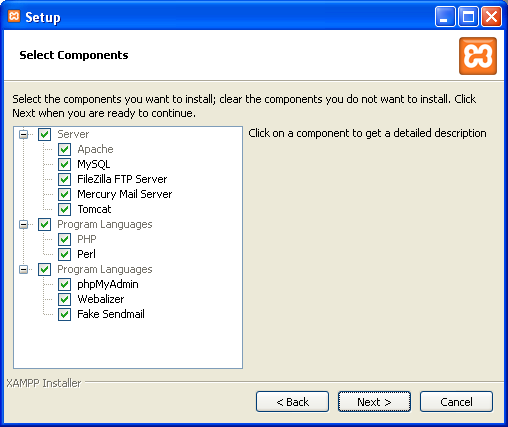
\includegraphics[width=1\textwidth]{01-03-01-002-select-comp}
		\caption{Pemilihan Komponen}
		\label{fig:01-03-01-002}
	\end{figure}
	
	\item Selanjutnya adalah penetapan \textit{folder} instalasi, akan ditaruh dimana hasil instalasi dari XAMPP ini. Tampilannya seperti pada gambar \ref{fig:01-03-03-003} berikut ini :
	
	\begin{figure}[H]
		\centering
		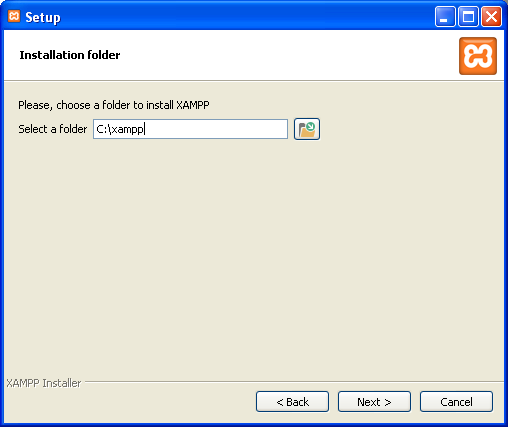
\includegraphics[width=1\textwidth]{01-03-01-003-inst-folder}
		\caption{Pemilihan \textit{Folder} Instalasi}
		\label{fig:01-03-01-003}
	\end{figure}
	
\end{enumerate}